\setcounter{section}{-1}

\hypertarget{introduction-video}{%
\section{Introduction Video}\label{introduction-video}}

24 lecture course. 
Full notes will be provided on moodle, small typefont indicates an aside, either because the material is non examinable or will be covered in greater detail in a later course.

Four example sheets.

\hypertarget{schedule}{%
\subsection{Schedule}\label{schedule}}

\begin{enumerate}
\def\labelenumi{\arabic{enumi}.}
\tightlist
\item
  Basic Calculus (5 lectures)
\item
  First-order linear differential equations (2)
\item
  Nonlinear first-order differential equations (4)
\item
  Higher-order linear differential equations (8)
\item
  Multivariate functions: applications (5)
\end{enumerate}

\hypertarget{introduction}{%
\subsection{Introduction}\label{introduction}}

They describe the rate of change of the \textcolor{red}{dependent variable} wrt the \textcolor{red}{independent variable}.

\begin{example}[Newton's 2nd law] ~\vspace*{-1.5\baselineskip}
\begin{align*}
  m \frac{d^2 x}{d t^2} = F
\end{align*}
If \(F\) depends only on \(t\), then we can simply integrate twice. However, if \(F\) is a function of \(x\) (such as a charged particle in a electric field which varied over space).
\end{example}

\textbf{Applied course} - emphasises \textcolor{red}{methods} and \textcolor{red}{results} rather than \textcolor{red}{proof} or \textcolor{red}{existence}.

\hypertarget{limits}{%
\subsection{Limits}\label{limits}}

\begin{itemize}
\item
  Informally, if \(\lim_{x \to x_0} f(x) = A\), then \(f(x)\) can be made arbitrarily close to \(A\) by making \(x\) sufficiently close to \(x_0\)

  \begin{itemize}
  \tightlist
  \item
    Note, does not require \(f(x_0)\) to equal \(A\) (or even to exist) -- a limit is a statement about the behaviour of a function in the vicinity of \(x_0\), but not at that point.
  \end{itemize}
\item
  More formally, for a function \(f(x)\) defined on some open interval containing \(x_0\) (but not necessarily at \(x_0\)), \(\lim_{x \to x_0} f(x) = A\) means that

  \begin{itemize}
  \tightlist
  \item
    for any \(\epsilon > 0\), there exists \(\delta >0\) such that \(|f(x) - A| < \epsilon\) for all \(0 < |x - x_0| < \delta\).
  \item
    Right hand limit, for example, defined similarly but with \(0 < |x - x_0| < \delta\) replaced with \(0 < x - x_0 < \delta\). A similar procedure can be done for left hand limits
  \end{itemize}

  \begin{figure}[h!]
    \centering 
    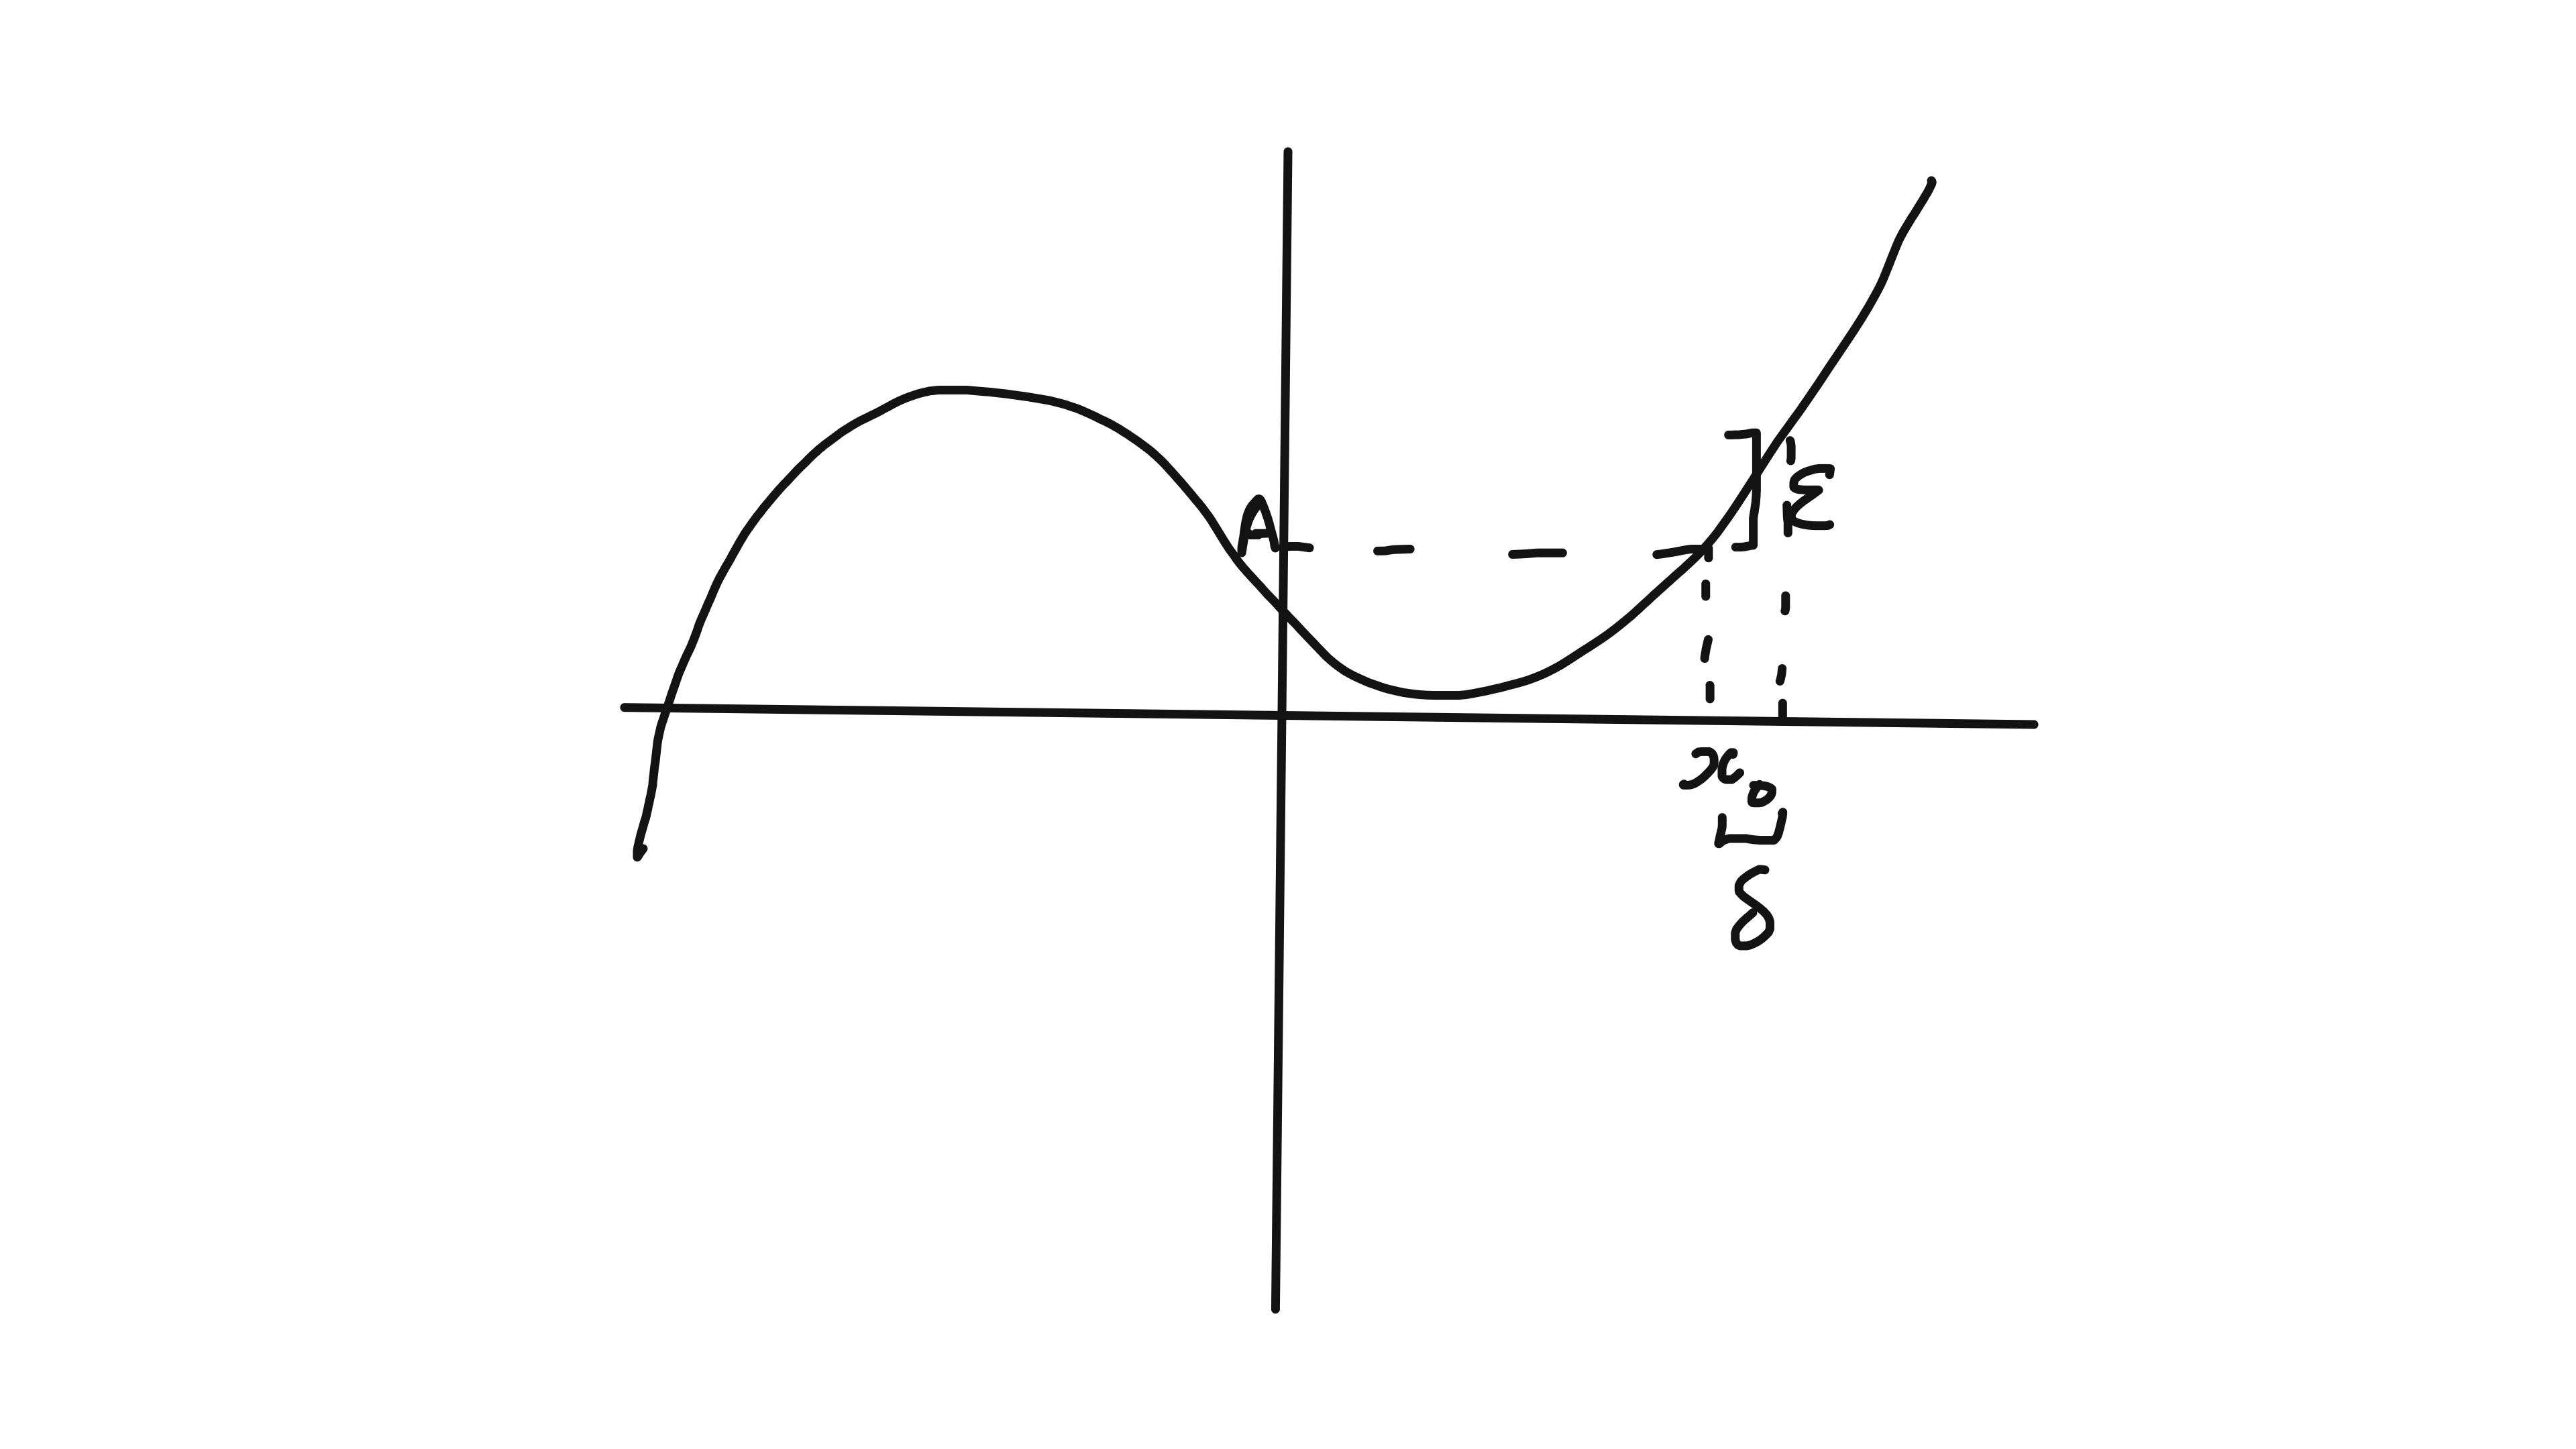
\includegraphics{figures/1}
    \caption{Right hand limit}
  \end{figure} \label{fig:1}
  
\item
  We can also define limits at infinity, e.g.~\(\lim_{x \to x_0} f(x) = A\) means that

  \begin{itemize}
  \tightlist
  \item
    for any \(\epsilon > 0\), there exists \(X >0\) such that \(|f(x) - A| < \epsilon\) for all \(x > X\).
  \end{itemize}
\end{itemize}

\hypertarget{properties}{%
\subsubsection{Properties}\label{properties}}

\begin{itemize}
\tightlist
\item
  If \(f(x)\) has a limit at a point, it is unique
\item
  If \(\lim_{x \to x_0} f(x) = A\) and \(\lim_{x \to x_0} g(x) = B\), then:

  \begin{itemize}
  \tightlist
  \item
    \(\lim_{x \to x_0} [f(x) + g(x)] = A + B\)\\
  \item
    \(\lim_{x \to x_0} [f(x)g(x)] = AB\)\\
  \item
    \(\lim_{x \to x_0} [f(x) / g(x)] = A / B\). If \(B = 0\), the limit of the quotient does not exist if \(A \neq 0\), but \textcolor{red}{may} exist in the \textcolor{red}{indeterminate} case \(A = B = 0\)
  \end{itemize}
\end{itemize}

These properties will be proved carefully in the Analysis 1 course next term, but will be used as without proof in this course.

\hypertarget{proof-of-uniqueness-of-limits}{%
\subsubsection{Proof of uniqueness of limits}\label{proof-of-uniqueness-of-limits}}

Suppose that \(\lim_{x \to x_0} f(x) = A\) \textcolor{red}{and} \(\lim_{x \to x_0} f(x) = B\).
In terms of our epsilon-delta definition, this means that for any \(\epsilon > 0\) there exists \(\delta_A > 0\) and \(\delta_B > 0\) such that
\begin{align*}
  &\text{for }0 < |x -x_0| < \delta_A,\ |f(x) - A| < \epsilon / 2 \text{, where } \epsilon / 2 \text{ is an arbitrary positive quantity.} \\
  \color{red}{and} \ &\text{for } 0 < |x -x_0| < \delta_A,\ |f(x) - B| < \epsilon / 2
\end{align*}
Now let \(\delta = min(\delta_A, \delta_B)\) and consider \(0 < |x -x_0| < \delta\) - follows that
\begin{align*}
  |A - B| &= |[A - f(x)] - [B - f(x)]| \\
  &\leq |A - f(x)| + |B - f(x)| \\
  &\leq \epsilon
\end{align*}
Since this holds \textcolor{red}{for all} \(\epsilon > 0\), we must have \(A = B\).